\documentclass[11pt]{article}
\usepackage[utf8]{inputenc}
\usepackage[T1]{fontenc}
\usepackage{graphicx}
\usepackage{grffile}
\usepackage{longtable}
\usepackage{wrapfig}
\usepackage{rotating}
\usepackage[normalem]{ulem}
\usepackage{amsmath}
\usepackage{textcomp}
\usepackage{amssymb}
\usepackage{capt-of}
\usepackage{hyperref}
\usepackage{minted}
\author{Student: Your Name and EID Here \\ Professor: Mohit Tiwari \\ TA: Austin Harris \\ Department of Electrical \& Computer Engineering \\ The University of Texas at Austin}
\date{\today}
\title{EEw382N Security Laboratory Exercise X Report}
\hypersetup{
 pdfauthor={Student: Your Name and EID Here \\ Professor: Mohit Tiwari \\ TA: Austin Harris \\ Department of Electrical \& Computer Engineering \\ The University of Texas at Austin},
 pdftitle={EEw382N Security Laboratory Exercise X Report},
 pdfkeywords={},
 pdfsubject={},
 pdfcreator={},
 pdflang={English}}
\begin{document}

\maketitle
\section{Problem 1}
\label{sec:prob-1}
Nam dui ligula, fringilla a, euismod sodales, sollicitudin vel, wisi. Morbi
auctor lorem non justo. Nam lacus libero, pretium at, lobortis vitae, ultricies
et, tellus. Donec aliquet, tortor sed accumsan bibendum, erat ligula aliquet
magna, vitae ornare odio metus a mi. Morbi ac orci et nisl hendrerit mollis.
Suspendisse ut massa. Cras nec ante. Pellentesque a nulla. Cum sociis natoque
penatibus et magnis dis parturient montes, nascetur ridiculus mus. Aliquam
tincidunt urna. Nulla ullamcorper vestibulum turpis. Pellentesque cursus luctus
mauris.

Example Equation~\ref{eq:example} shows X.

\begin{align}
f(x) = \frac{x^3}{\epsilon_0}
\label{eq:example}
\end{align}

\section{Problem 2}
\label{sec:prob-2}
Example Figure \ref{fig:rocc-encoding} shows X. Example reference to paper~\cite{Brasser17}.

\begin{figure}[htbp]
\centering
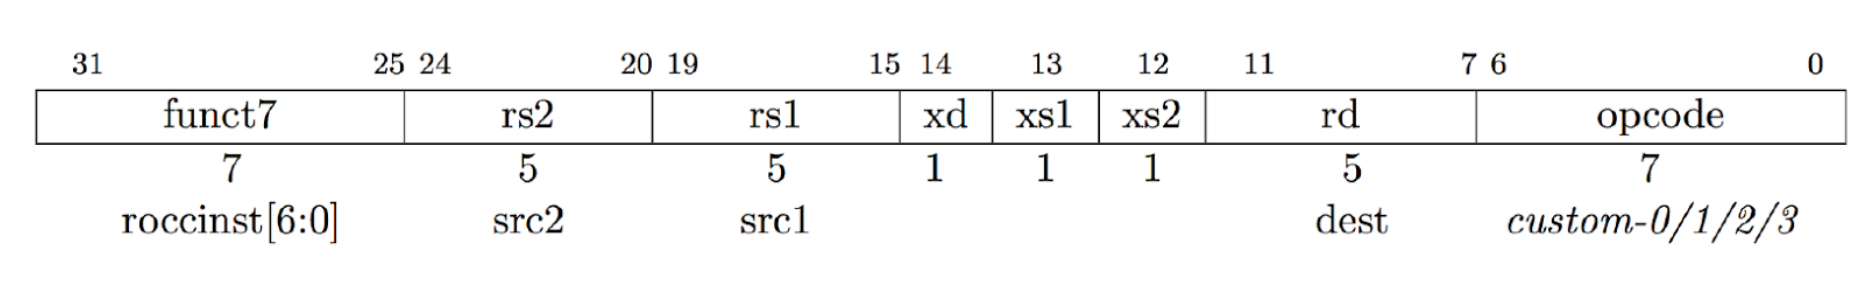
\includegraphics[width=.9\linewidth]{./rocc-encoding.png}
\caption{\label{fig:rocc-encoding}
The RoCC Accelerator Instruction Encoding}
\end{figure}
\section{Problem 3}
\label{sec:prob-3}
Nulla malesuada porttitor diam. Donec felis erat, congue non, volutpat at,
tincidunt tristique, libero. Vivamus viverra fermentum felis. Donec nonummy
pellentesque ante. Phasellus adip- iscing semper elit. Proin fermentum massa ac
quam. Sed diam turpis, molestie vitae, placerat a, molestie nec, leo. Maecenas
lacinia. Nam ipsum ligula, eleifend at, accumsan nec, suscipit a, ipsum. Morbi
blandit ligula feugiat magna. Nunc eleifend consequat lorem. Sed lacinia nulla
vitae enim. Pellentesque tincidunt purus vel magna. Integer non enim. Praesent
euismod nunc eu purus. Donec bibendum quam in tellus. Nullam cursus pulvinar
lectus. Donec et mi. Nam vulputate metus eu enim. Vestibulum pellentesque felis
eu massa.

\begin{minted}{c++}
  int main() {
    printf("Hello World");
    return 0;
  }
\end{minted}

\section{Conclusion}
\label{sec:conclusion}
Please provide feedback so we can improve the labs for the course. How many
hours did the lab take you? Was this lab boring? Did you learn anything? Is
there anything you would change? Feel free to put anything here, but leaving it
blank will result in the loss of points.

\bibliography{bibliography}
\bibliographystyle{ieeetr}
\end{document}
